\chapter{Motor Control Theory} \label{chap:theory}

In this chapter, we will review some theoretical principles that concern us regarding motor control. First, we will review the physical principles that rule over the electric motors and we will explain the different motor technologies and its configurations, focusing in the \acf{PMAC} motors. Later, we will review the motor drives, the configuration of a driver and the different driving techniques for the \ac{PMAC} motors. Finally, we will explain the control methods that can be applied to them.

Most of the theory in this chapter was taken from the book \citetitle{sistemi_di_controllo:2007}, by \citeauthor{sistemi_di_controllo:2007}, \citeyear{sistemi_di_controllo:2007} and from the compilation \citetitle{AC_drives}, by \citeauthor{AC_drives}, \citeyear{AC_drives}.


\section{Electric Motor}

An electric motor is an electric machine that transforms electrical power (product between voltage and current):

\begin{equation}
	\label{eq:e_elec}
	P_{electrical} = V \cdot I
\end{equation}

into mechanical power (product between torque and angular speed):

\begin{equation}
	\label{eq:e_mech}
	P_{mechanical} = T \cdot \omega
\end{equation}

by means of the electromagnetic phenomena that takes place inside the motor, which is explained by the physical principles mentioned in this chapter.

\subsection{Physical Principles} \label{physical_principles}

The generation of torque in electric motors is based in the interaction of two magnetic fields, one generated by magnets or windings placed in the stator and the other one generated by magnets or windings placed in the rotor as seen in Figure \ref{fig:motor_assembly}.

\begin{figure}[htbp]
\centering
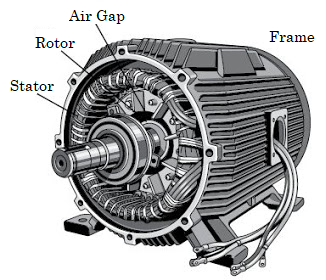
\includegraphics[width=8cm]{Images/motor_assembly.png} 
\caption[Partially Assembled Motor]{Partially Assembled Motor. An electric motor consists mainly in three parts: a rotor, which moves due to the electromagnetic interaction; a stator, the body of the motor; and a frame, which holds the rotor and the stator together. The air gap is the space betweeen the rotor and the stator, where the electromagnetic interaction takes place (\citetitle{basic_components}, \citeyear{basic_components}).}
\label{fig:motor_assembly}
\end{figure}

The physical laws that rule over the electric motor are mainly four: The Lorentz’s Law, which helps us define the torque generated by an electric charge moving inside a magnetic field; Faraday’s Law of Electromagnetic Inductance and the Lenz’s Law, which explain the generation of the \acf{BEMF} in the motor coils depending on the speed of the rotor and the influence of the magnetic field generated due to this BEMF respectively; and the Ampere-Laplace Law, which allows us to calculate the magnetic field of a current loop and the mechanical interaction between two magnetic fields.

\begin{description}

\item[Lorentz's Law] defines a force $F$, which acts over an electric charge $q$ moving with a speed $v$ inside a magnetic field with intensity $B$ as seen in Figure \ref{fig:lorentz_law}:

\begin{equation}
	\label{eq:force_1}
	F = q v \times B
\end{equation}

By defining a current $I$ passing through a conductor with length $l$ we can transform Equation \ref{eq:force_1} into Equation \ref{eq:force_2}:

\begin{equation}
	\label{eq:force_2}
	F = l I \times B
\end{equation}

Considering the current $I$ flowing through a conductive loop as the one in Figure \ref{fig:lorentz_law} with sides lengths $l$ and $h$ we can see that there is a force $F$ generated in the direction of the cross product of the current $I$ and the magnetic field $B$. The maximum force $F$ is generated in the sides of the loop where the direction of the current $I$ is perpendicular to the direction of the magnetic field $B$ ($ab$ and $cd$), while on the other two sides ($ad$ and $bc$) the forces generated are cancelled with each other due to the direction of the current respect to the magnetic field.

\begin{figure}[htbp]
\centering
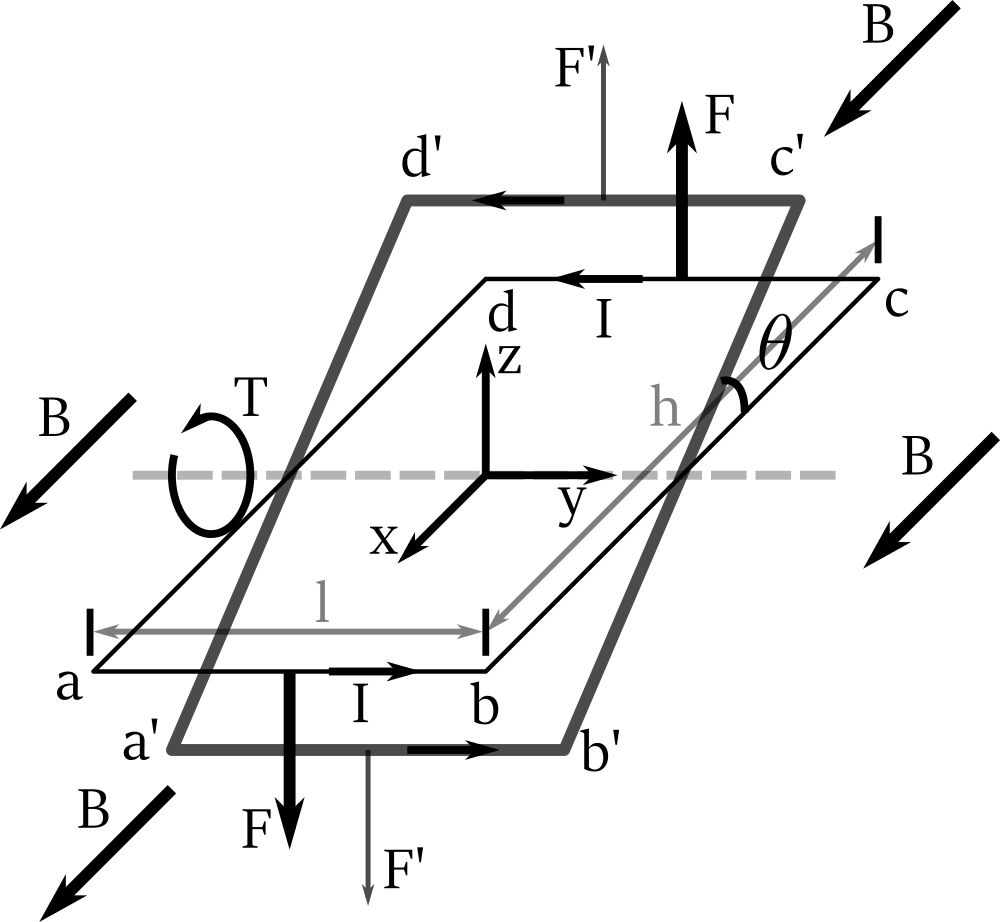
\includegraphics[width=8cm]{Images/lorentz_law.png} 
\caption[Lorentz's Law Diagram]{Visual explanation of the interaction of the current $I$ and the magnetic field $B$ generating a force $F$ and, consecuently, a torque $T$ around the $y$ axis (\citeauthor{sistemi_di_controllo:2007}, \citeyear{sistemi_di_controllo:2007}).}
\label{fig:lorentz_law}
\end{figure}

Since the forces $F$ generated on the sides $ab$ and $cd$ have the same magnitude but different direction, they create a torque $T$ around the $y$ axis defined by the magnetic field, the current and by the length of the sides of the loop as:

\begin{equation}
	\label{eq:torque_1}
	T = I h l B \cos \theta
\end{equation}

We can see in Figure \ref{fig:lorentz_law} and in Equation \ref{eq:torque_1} that when the angle $\theta$ between the sides $ad$ or $bc$ and the direction of the magnetic field $B$ is $\pi / 2$ radians, the torque $T$ is zero and when the angle $\theta$ is zero or $\pi$ radians, the torque reaches its maximum possible value. 

The dependency of the torque created by the interaction of the current and the magnetic field on the angle between these two physical quantities introduces the need of changing the direction of the magnetic field or the direction of the current, hence, the polarity of the loop, to maintain the loop spinning and a non-zero torque.

\item[Faraday’s Law of Electromagnetic Induction] states that
\blockquote{In every circuit under the effect of a magnetic field, an electromotive force is induced equal to the derivative respect to the time of the magnetic flux passing though the circuit, with negative sign. (\citeauthor{emWaves:1968}, \citeyear{emWaves:1968})}

therefore, by indicating with $E$ the electromotive force and with $\phi _{m}$ the magnetic flux, we have:

\begin{equation}
	\label{eq:em_1}
	E = - \frac{\mathrm{d} \phi _{m}}{\mathrm{d} t}
\end{equation}

If we consider a case like the one in Figure \ref{fig:lorentz_law} we can calculate the magnetic flux passing though the loop as:

\begin{equation}
	\label{eq:mf_1}
	\phi _{m} = B \cdot u_{N} S = B \cdot u_{N} h l = h l B \sin \theta 
\end{equation}

where $S$ is the surface of the loop and $u_{n}$ is the direction normal to the plane of the loop. Therefore, we get an induced electromotive force of:

\begin{equation}
	\label{eq:em_2}
	E = - \omega h l B \cos \theta
\end{equation}

where $\omega$ is the angular speed of the loop. We can see, comparing Equation \ref{eq:em_2} and Equation \ref{eq:torque_1}, that the induced electromotive force depends on the angular speed in the same way than the acting torque depends on the current.

\item[Lenz's Law] can be explained after the explanation of the induced electromotive force. It states that the induced current in a loop has the direction that creates a magnetic field that opposes the change in magnetic flux through the area enclosed by the loop, therefore, the induced current tends to keep the magnetic flux $\phi _{m}$ from changing in the circuit.

If the rotation of the loop is generated by the circulation of a current inside a magnetic field, the induced electromotive force will try to oppose to the pass of the current, that’s why it’s normally referred to as \acf{BEMF}.

\item[Ampere-Laplace Law] is the last piece to understand the transformation of electrical energy into mechanical energy. It allows us to calculate the magnetic field generated by a closed loop conducting current in a point defined by a vector $p$ as:

\begin{equation}
	\label{eq:B_1}
	B(p) = \frac{\mu_{0}}{4 \pi} \oint I \frac{u_{t} \times u_{r}}{r^{2}}dl
\end{equation}

where $\mu_{0}$ is the vacuum magnetic permeability constant, $I$ is the current circulating through the loop, $u_{t}$ is the versor with direction of the current in the infinitesimal element $dl$ and $u_{r}$ and $r$ are versor and module that define the point $p$ respect to the infinitesimal element of the loop.

Given that the magnetic fields can be generated both by permanent magnets and by current circulation, the electromechanical conversion is obtained due to the interaction of two magnetic fields according to the alignment principle:

\blockquote{In a region of space which hosts two magnetic fields, there is a mechanical action that tends to align both fields. (\citeauthor{sistemi_di_controllo:2007}, \citeyear{sistemi_di_controllo:2007})}

So, if we consider the loop from Figure \ref{fig:lorentz_law} and Equation \ref{eq:B_1}, we can see that there is a magnetic field generated around the loop as seen in Figure \ref{fig:alignment}, and due to the alignment principle, we will get the strongest coupling torque when the magnetic fields are perpendicular to each other.

\begin{figure}[htbp]
\centering
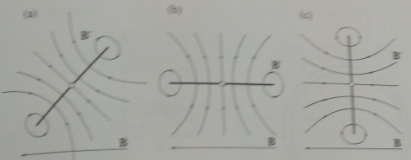
\includegraphics[width=8cm]{Images/alignment.png} 
\caption[Alignment Principle]{Visual explanation of the alignment principle. The alignment torque is the largest in the configuration of figure B and nule in the configuration of figure C.}
\label{fig:alignment}
\end{figure}

In the case of electrical motors, there are two different magnetic fields generated in the airgap due to the permanent magnets or to the windings placed in the stator and the rotor which can be considered in radial direction, described by two magnetic fields $B_{r}(\theta,t)$ and $B_{s}(\theta,t)$, from which interaction we get the electromechanical conversion, since we have the generation of a torque which tends to align the two fields angles where they have the largest intensity. The alignment torque will be an expression of the type:

\begin{equation}
	\label{eq:torque_2}
	\tau_{m} = k B_{r} B_{s} \sin \delta
\end{equation}

where $\delta$ is the de-phasing angle between the two fields and the maximum torque will be when $\delta = \pi / 2$.

\end{description}

In conclusion, by feeding the windings in the right way, we look forward to having a constant 90° de-phase between the two magnetic fields in aims to obtain the maximum torque generation.

In the case of the \acf{DC} motor, the perpendicularity condition is maintained by a polarity commutating structure attached to the rotor which is connected to the windings that generate the rotor magnetic field that tries to align itself to the magnetic field of the permanent magnets attached to the stator. This commutating system is connected to the power supply by metallic brushes that energyse the motor until it reaches a certain angular position and the commutating lead changes to the next one, changing the polarity of the windings. Therefore, the torque obtained is independent from the position of the rotor and it’s proportional to the amplitude of the power source.

\begin{figure}[htbp]
\centering
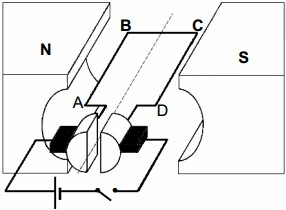
\includegraphics[width=8cm]{Images/dc_motor.png} 
\caption[DC Motor Scheme]{Basic schematic representation of the \ac{DC} motor using the same loop represented in Figure \ref{fig:lorentz_law}}
\label{fig:dc_motor}
\end{figure}

Brushless motors, which will be explained later in this chapter, the perpendicularity condition is maintained by feeding in the right time the windings in function of the angular position of the rotor $\theta$, which is one of the main goals to be achieved and explained in this work.

\section{PMAC Motors}

The \acf{PMAC} motor is a kind of electrical motor that doesn't need the mechanical commutators mentioned in \ref{physical_principles} to be driven as in the case of the DC motor, but its windings need to be energysed in a specific way to function correctly. Since it doesn't need the mechanical commutators, it also doesn't need the brushes that energyse the windings, so it can be said that it's a brushless motor. As seen in Figure \ref{fig:brushless_section}, there are permanent magnets attached to its rotor and the coils are winded into its stator in a three-phase configuration.

\begin{figure}[htbp]
	\centering
	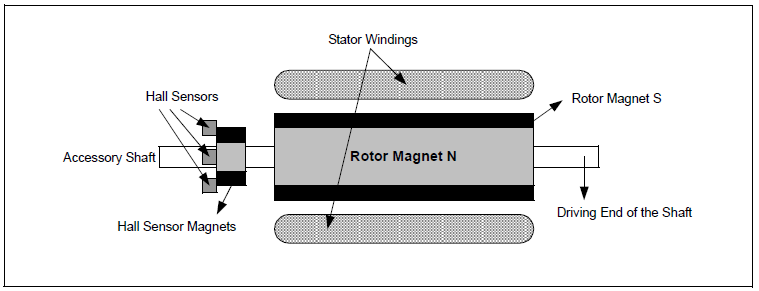
\includegraphics[width=12cm]{Images/brushless_section.png} 
	\caption[Brushless Motor Transverse Section]{Brushless motor transverse section (\citeauthor{microchip}, \citeyear{microchip}).}
	\label{fig:brushless_section}
\end{figure}

These three phases are fed alternativelly in such a way that the magnetic field, generated by the relative currents passing through the coils, should always be orthogonal and synchronous to the magnetic field generated by the rotor's permanent magnets. The characteristics mentioned above give the name to this kind of motors. 

To maintain the synchronization, it's necessary to commute, by means of an inverter as the one represented in Figure \ref{fig:inverter_1}, the currents in the windings of the stator, taking as a reference the angular position of the rotor, which must be obtained by a sensor.

The number of commutations needed to generate one revolution of the rotor is determined by the number of times that each phase coil is winded in the stator. For example, if each phase coil of the three phase system is winded only once, one commutation would be enough to generate one revolution, but if each phase coil is winded 6 times, we would need to commutate the power supply of the coils six times to generate one revolution. This ratio is called \acf{PP}. Normally, the \ac{PMAC} motors have many \ac{PP} (six or more) in order to have a lower torque ripple since the alignment of the magnetic fields would be every $360\degree/(\ac{PP} \times \Phi_{N})$ degrees of the rotor. For the study on the electromechanical conversion, the angular position of the rotor is substituted by an electrical angular position, which is controlled by the commutator and is defined by:

\begin{equation}
	\label{eq:pole_pairs}
	\theta_{electrical} = \ac{PP} \theta_{mechanical}
\end{equation}

which also represents a relationship between the mechanical speed of the rotor and the electrical speed of commutation, which is defined by the commutation frequency:

\begin{equation}
	\label{eq:pole_pairs}
	\omega_{electrical} = f_{commutation} = \ac{PP} \omega_{mechanical}
\end{equation}

so, for example, if we have a motor with 6 \ac{PP} and we want to drive it at $1 kHz$, we must commutate the polarity of the inverter at $f_{commutation} = \ac{PP} \omega_{mechanical} = (6) (1 kHz) = 6 kHz$.

\begin{figure}[htbp]
	\centering
    \subfloat[2 Pole Pairs\label{subfig-1:2_pole}]{%
    	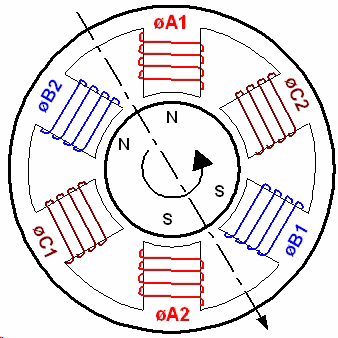
\includegraphics[width=0.3\textwidth]{Images/2_pole.png}
    }
    \hfill
    \subfloat[2 Pole Pairs\label{subfig-2:4_pole}]{%
      	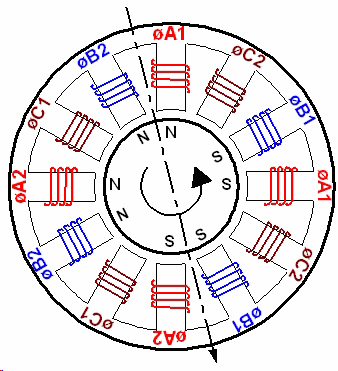
\includegraphics[width=0.3\textwidth]{Images/4_pole.png}
    }
    \hfill
    \subfloat[2 Pole Pairs\label{subfig-3:6_pole}]{%
      	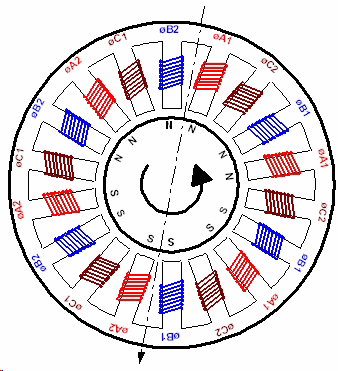
\includegraphics[width=0.3\textwidth]{Images/6_pole.png}
    }
    \caption{Different pole pair configurations}
    \label{fig:pole_pairs}
    %https://www.basilnetworks.com/article/motors/brushlessmotors.html
\end{figure}

The main characteristics that make the brushless motor a better option for some applications than the \ac{DC} motor are the following:
\begin{itemize}
	\item better weight-to-power ratio,
	\item a more linear acceleration,
	\item a low inertia,
	\item a higher reliability,
	\item smaller dimension,
	\item reduced need for maintenance,
	\item high rotation speed,
	\item ideal for working in hostile environments
\end{itemize}

There are two disadvantages to this motor technologies: the first one is the need of a rotation sensor; the second one is the need of a complex logic to commutate the currents flowing through the coils. Both of these disadvantages are mainly reflected in a higher price respect to the \ac{DC} motor.

It is possible to identify mainly two types of brushless motors. The first one is the \acf{BLDC} motor, which has a rotor position feedback that is not continuous, since the position of the rotor is given every 60 electrical degrees and its feed in blocks of 120 electrical degrees by simply alternating the voltage in the inverter, and due to these alimentation in blocks, the driving is rectangular, so the ideal \ac{BEMF} is trapezoidal. The second type of brushless motors needs a continuous rotor position feedback to feed the motor with sinusoidal current, obtained by \acf{PWM} of the \ac{DC} bus, therefore the ideal \ac{BEMF} is sinusoidal, which generates a lower torque ripple than the trapezoidal one, but needs a more complex control method.

\subsection{BLDC Motors}

The stator winding for each phase of the \ac{BLDC} motor consists of a uniform distribution of turns over $N=\ac{PP}$ sectors of a width equal to 60\degree. The magnets attached to the stator cover an arc of 180\degree, and at any instant, each magnet interacts, for 120\degree, with an arc of stator conductor carrying current. Due to this discrete interaction every 120\degree, the three-phase switching between the currents of the stator should happen when the edge of the magnet attached to the rotor reaches the boundary between windings every 60\degree.

The boundary of the rotor magnets with respect to the windings position is detected by three sensors, one every 60\degree, which send a signal to the driving circuit to change the polarity of the coils depending on the actual value of the three sensors and on the desired direction. The sensors to detect the angular position will be explained in \ref{section:drives} and the driving sequences will be explained in \ref{section:driving_methods}.


\subsection{PMSM Motors}

The stator is fitted with three-phase windings with $N=\ac{PP}$ turns of each phase distributed sinusoidally around the periphery. If the stator windings are feed by sinusoidal currents, there is a linear current density around the stator periphery

\section{Motor Drives}\label{section:drives}

Some explanation about how motor drives are conformed...\\

\subsection{Inverter}

The commutation of the polarities in the windings of the \ac{PMAC} motors is done by means of a three-phase inverter. The inverter used in \ac{PMAC} motors and the use of recirculation diodes avoids the need of the mechanical commutation used in the \ac{DC} motors, which creates sparks between the commutator and the brushes due to the discharge of the electromagnetic energy stored in the windings of the rotor. This characteristic limits the use of \ac{DC} motors to applications where sparks don't represent a latent danger. Also the \ac{DC} motors need constant maintenance since the brushes need to be replaced periodically, while brushless motors can run for years without the need of changing any component.

\begin{figure}[htbp]
\centering
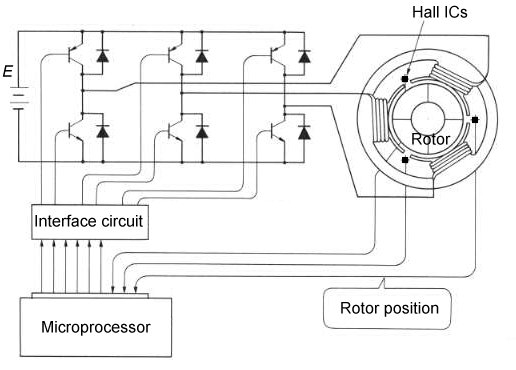
\includegraphics[width=10cm]{Images/inverter_1.png} 
\caption[Three-Phase Inverter]{Schematic representation of the three-phase inverter circuit needed to drive a brushless motor(\citeauthor{microchip}, \citeyear{microchip}).}
%http://www.ewh.ieee.org/soc/es/May2001/02/FIG2.JPG
\label{fig:inverter_1}
\end{figure}

The use of recirculation diodes is necessary to avoid damage in the transistors due to the overvoltage generated by the current transients in the windings $L dI/dt$ that takes place between the switches of a same branch of the inverter while switching from one state to another. For example, when a transistor is suddenly turned off, the current flowing through the coils doesn't instantly dissapear, but instead it recirculates through the diodes until it vanishes.

\subsection{Peripherals}




\section{PMAC Motors Driving Methods}\label{section:driving_methods}

\subsection{Trapezoidal Drive}

\subsection{Sinusoidal Drive}




\section{Control Methods}

\subsection{Speed Control}

\subsection{Torque Control}

\subsection{Field Oriented Control}

\subsection{Speed Control with Field Oriented Control}



